\section{On data compression: Entropy of a source}
Let's imagine a source which emits symbols from the alphabet $A$ with some frequency, we define it's \emph{entropy} with:
$$
    H_0 = \sum_{\sigma \in A} p_{\sigma} log_2 \frac{1}{p_{\sigma}}
$$
in which:
\begin{itemize}
    \item $p_{\sigma}$ is the probability of emitting the symbol $\sigma$, so $0 \leq p_{\sigma} \leq 1$;
    \item $H_0 \geq 0$ because $log_2 \frac{1}{p_{\sigma}} \geq 0$;
    \item 0 in $H_0$ stands for entropy of single symbol;
    \item the unit of measure is \emph{bits}.
\end{itemize}

$H_0$ is a convex function and it's maximum is when all probabilities are equals, so if:
$$
    p_{\sigma} = \frac{1}{|A|}
$$
so:
$$
    H_0 = \sum_{\sigma \in A} p_{\sigma} log_2 \frac{1}{p_{\sigma}} \leq \sum_{\sigma \in A} \left( \frac{1}{|A|} \right) log_2 \frac{1}{\frac{1}{|A|}} = |A| \cdot \left( \frac{1}{|A|} \right) log_2 |A| = log_2 |A|
$$
So we got a higher bound for the entropy of a source.

Let's try to give an interpretation for that formula: suppose that $X$ is a random variable that assumes the value $log_2 \frac{1}{p_{\sigma}}$ with probability $p_{\sigma}$, then:
$$
    \mathbb{E}[X] = \sum_{\sigma \in A} p_{\sigma} \cdot \left(  log_2 \frac{1}{p_{\sigma}} \right)=
$$
We can interpret entropy as the average of a source emitting symbol $log_2 \frac{1}{p_{\sigma}}$ with probability $p_{\sigma}$, so if $log_2 \frac{1}{p_{\sigma}}$ is the information content of the symbol $\sigma$ then $H_0$ is the average of information content.

Ex: if $p_A = 1$ and $p_B = 0$ then:
\begin{itemize}
    \item $p_A \cdot log_2 \frac{1}{p_A} = 0$: if the source always sends A then there is no content;
    \item $p_B \cdot log_2 \frac{1}{p_B} \xrightarrow{} \infty$: if the source says a very rare symbol we gather a lot of information.
\end{itemize}

\subsection{Shannon's theorem}
Any \emph{prefix-free code} for the source $S$ takes an \emph{average} of bits per symbol $\geq H_0$, so $H_0$ is a lower bound.

A prefix-free code is an encoding in which there is no symbol which is a prefix of another symbol.

Ex: $a = 0, b = 01, c = 1$: we have that $a$ is prefix of $b$, so if we read the bits 01 we don't know if it's the encoding of $b$ or $ac$.


$a = 0, b = 10, c = 111$ is prefix-free, let's calculate the average code length with $p_a = \frac{1}{4}, p_b = \frac{1}{2}, p_c = \frac{1}{4}$:
$$
    \mathbb{E}[|cw(\sigma)|] = \sum_{\sigma \in A} p_{\sigma} \cdot |cw(\sigma)| = \frac{1}{4} \cdot 1 + \frac{1}{2} \cdot 2 + \frac{1}{4} \cdot 3 = \frac{1}{4} + 1 + \frac{3}{4} = 2 \frac{bits}{symbol}
$$
with $cw(\sigma)$ the codeword of $\sigma$, so the encoding.
Is it a good encoding or not? Let's check the lower bound:
$$
    \frac{1}{4} log_2 (4) + \frac{1}{2} log_2 (2) + \frac{1}{4} log_2 (4) = \frac{1}{2} \cdot 2 + \frac{1}{2} \cdot 1 + \frac{1}{4} \cdot 2 = \frac{1}{2} + \frac{1}{2} + \frac{1}{2} = \frac{3}{2} = 1.5 \frac{bits}{symbol}
$$
So the code we used is not optimal since it's higher than the lower bound.
An optimal encoding could be: $a = 00, b = 1, c = 01$:
$$
    \mathbb{E}[|cw(\sigma)|] = \frac{1}{4} \cdot 2 + \frac{1}{2} \cdot 1 + \frac{1}{4} \cdot 2 = \frac{1}{2} + \frac{1}{2} + \frac{1}{2} = \frac{3}{2} = 1.5 \frac{bits}{symbol}
$$

\subsection{Golden rule of data compression}
$$
    p_{\sigma} > p_{\sigma'} \implies |cw(\sigma)| \leq |cw(\sigma')|
$$
the bigger the probability, the shorter the symbol encoding.

Who gives us the probabilities and the encoding?
If the message $T$ is known we can count the appearances of each element and we can use:
$$
    p_{\sigma} \approx freq(\sigma) = \frac{occ(\sigma)}{|T|}
$$
this model is called \emph{semi-static model}.

There is also a \emph{dynamic model} in which we start with each symbol with equal probability and at each new emitted symbol we adjust those probabilities.
We use this technique in streaming model and each time we change the encoding.

\section{Integer coding}
Given $S = s_1, s_2, s_3, \_, s_n$ with $s_i \in \mathbb{N}$ and $s_i < s_{i+1}$ we define the \emph{gap sequence} as:
$$
    S' = s_1, (s_2 - s_1), (s_3 - s_2), \_
$$
NB: the property $s_i < s_{i+1}$ doesn't lack of generality because we can always find a transformation from every $S$ to a sequence with this property, for example we can use the \emph{sum sequence} in which each element is the sum of all the previous one.

NB: $s_i \in \mathbb{N}$ doesn't lack of generality because we can exploit the numerability of $\mathbb{Z}$ to create a map $\mathbb{Z} \xrightarrow{} \mathbb{N}$:
$$
\begin{cases}
    2x & \text{ if $x \geq 0$ } \\
    2|x| + 1 & \text{ if $x < 0$ } \\
\end{cases}
$$

So our problem is: how to represent $S$ with the least number of bits?

Es: $S = 3, 5, 6 \implies S' = 3, 2, 1$, from $S$ to $S'$ ad vice versa is straightforward.

Now that $S'$ has some repetitive element we can exploit those repetitions to compress data.

\subsection{Naive encoding}
Given $S = s_1, s_2, \_, s_n$ with $s_i < s_{i+1}$, we pick $S^* = s_n + 1$ we encode each $s_i$ in a fixed-len of $\lceil log_2 S^* \rceil$ bits.
It's simple but it's a waste of space.

\subsection{Unary encoding}
Given $x \geq 1$ we define:
$$
    U(x) = 0^{x-1} 1
$$
Ex: $U(1) = 1, U(2) = 01, U(3) = 001$.

\subsubsection{Optimal distribution}
This approach is stupid but it's optimal for some distributions: when $|cw(\sigma)| = log_2 \frac{1}{p_{\sigma}}$, it happens when:
$$
    |U(\sigma)| = log_2 \frac{1}{p_{\sigma}} \implies \sigma = log_2 \frac{1}{p_{\sigma}} \implies 2^{\sigma} = \frac{1}{p_{\sigma}} \implies p_{\sigma} = \frac{1}{2^{\sigma}}
$$
So if distribution of $\sigma$ is exponentially decreasing unary code is optimal!

NB: we used Shannon's theorem to derive the distribution which optimize our encoding.

\subsection{$\gamma$-code}
Given $x \geq 1$:
$$
    \gamma(x) = 0^{l-1} bin(x)
$$
with $l = |bin(x)| = \lceil log_2 (x+1) \rceil$ and $bin(x)$ the binary encoding.

Ex: $\gamma(9) = 000 1001$

It works because each $x$ starts with a 1 for sure (since $x \geq 1$), so $|\gamma(x)| = 2l-1 = 2 \lceil log_2 (x+1) \rceil - 1 \approx 2log_2 x -1$.
So $\gamma(x)$ is twice as long as $x$ but it's structure is useful because counting zeroes we can know how to decode: for example 0010100111010... we parse it:
\begin{itemize}
    \item 00: $len(00) = l-1$ so the number is long 3 bits;
    \item 101: the number is 5;
    \item 00: $len(00) = l-1$ so the number is long 3 bits;
    \item 111: the number is 7;
    \item 0: $len(0) = l-1$ so the number is long 2 bits;
    \item 10: the number is 2.
\end{itemize}

It's decoding time is slow because there is a variable part.

\subsubsection{Optimal distribution}
Let's recover the optimal distribution for this encoding:
$$
    |\gamma(x)| = log_2 \frac{1}{p(x)} \implies 2log_2 x - 1 = log_2 \frac{1}{p(x)} \implies
$$
$$
    2log_2 x = log_2 \frac{1}{p(x)} + 1 \implies 2log_2 x = log_2 \left( \frac{1}{p(x)} \cdot 2 \right) \implies
$$
$$
    log_2 x^2 = log_2 \left( \frac{2}{p(x)} \right) \implies x^2 = \frac{2}{p(x)} \implies p(x) = \frac{2}{x^2}
$$

\subsection{$\delta$-code}
Given $x \geq 1$:
$$
    \delta(x) = \gamma(l) bin(x)
$$
with $l = |bin(x)|$.

NB: $\delta(l)$ and not $\delta(l-1)$ because we can't encode 0 with $\delta$ so no encoding for 1.

Ex: $\delta(9) = 00100 1001$

NB: $\gamma(9) = 0001001$ is better than $\delta(9)$ but as $x$ increases $\delta$ starts to perform better.

Since $\gamma$-code was slow in decoding this is even slower. 

\subsubsection{Optimal distribution}
$$
    |\delta(x)| = |\gamma(l)| + l = 2log_2 l - 1 + l = l + 2log_2 l -1 = log_2 x + 2log_2 log_2 x - 1
$$
$$
    \implies |\delta(x)| = log_2 \left( \frac{1}{p(x)} \right) \implies p_x = \frac{2}{x}
$$

\subsection{Rice encoding}
It's an encoding useful when the values distribution is concentrated nearby a fixed value (like Gaussian distribution).
It's a parametric code for $k$:
$$
    R_k(x) = U(q) bin(r)
$$
with:
\begin{itemize}
    \item $q = \lfloor \frac{x-1}{2^k} \rfloor$: is the quotient;
    \item $r = x-1 - 2^k \cdot q$: is the remainder. 
\end{itemize}
Since $r < 2^k$, because it's a remainder, it stays on $k$ bits. 
$q$ instead can be 0 too so we use $U(q)$ which stays on $q+1$ bits.

Ex: $R_4(20) = $:
\begin{itemize}
    \item $q = \lfloor \frac{20-1}{2^4} \rfloor = \lfloor \frac{19}{16} \rfloor = 1 $;
    \item $r = 20-1-2^4\cdot 1 = 19-16 = 3$
\end{itemize}
$R_4(20) = 01 0011$.

It's decoding is slow since there is a variable length part.

\subsection{PForDelta}
We need codes with faster decoding time, for example codes aligned to byte.
PForDelta it's a blocked scheme with parameters $b$ and a base.

Given $S = 5, 4, 6, 7, 9, 15, 9, 20, 4$ we set as \emph{base} the minimum element and shift everything respect to it (called shift to 0) obtaining: $S = 1, 0, 2, 3, 5, 11, 5, 16, 0$.
We choose $b$ which is the number of bits used for compression, for example $b = 3$.
Then we create two types of elements:
\begin{itemize}
    \item ESC: an escape sequence, for example 111. 1 sequence;
    \item all the others. $2^b - 1$ sequences.
\end{itemize}
Then we compress data: if the number stays on $b$ bits and is different from ESC sequence, we memorize it as it is, otherwise we memorize it as it is in another sequence and put an ESC in the compressed sequence.

Ex: 001 | 000 | 010 | 011 | 101 | 111 | 101 | 111 | 000 is the compressed sequence and the uncompressed sequence must contain just the numbers 11 and 16 with naive encoding (maybe encoding on 8 bits or more).

This decoding is fast because we know the size of the compressed elements so the decoding strategy is immediate.

\subsubsection{Rule of thumb}
We need to choose $b$, a common strategy is to choose $b$ so that 90\% of $S$ is encoded in $b$ bits.

\subsection{Elias-Fano code}
We take into account increasing sequences: $S= 1, 4, 7, 18, 24, 26, 30, 31$, we define:
\begin{itemize}
    \item $u = s_n +1$: in this case 32;
    \item $b = \lceil log_2 u \rceil$: in this case 5, it should be enough to represent each element;
    \item $l = \lceil log_2 \frac{u}{n} \rceil$: in this case 2;
    \item $h = b-l = 3$
\end{itemize}
we split each number in low and high part:
\begin{table}[H]
    \centering
    \begin{tabular}{c|c|c|c|c}
        $i$ & $s_i$ & $bin(b)$ & $H(s_i)$ & $L(s_i)$ \\
        \hline
        1 & 1 & 00001 & 000 & 01 \\
        2 & 4 & 00100 & 001 & 00 \\
        3 & 7 & 00111 & 001 & 11 \\
        4 & 18 & 10010 & 100 & 10 \\
        5 & 24 & 11000 & 110 & 00 \\
        6 & 26 & 11010 & 110 & 10 \\
        7 & 30 & 11110 & 111 & 10 \\
        8 & 31 & 11111 & 111 & 11 \\
    \end{tabular}
    \caption{Elias-Fano algorithm}
\end{table}
we now have high and low parts.
We copy low parts one after the other:
$$
    L= 01 00 11 10 00 10 10 11
$$
$$
    |L| = l \cdot n = n \cdot \lceil log_2 \frac{u}{n} \rceil bits
$$

To build the sequence $H$ we count how many high parts there are for each combination and we represent those numbers in negative unary (unary encoding with bits flipped), so:
\begin{itemize}
    \item 10: because the configuration 000 appears once;
    \item 110: because the configuration 001 appears twice;
    \item 0: because the configuration 010 doesn't appear;
    \item 0: because the configuration 011 doesn't appear;
    \item 10: because the configuration 100 appears once;
    \item 0: because the configuration 101 doesn't appear;
    \item 110: because the configuration 110 appears twice;
    \item 110: because the configuration 111 appears twice.
\end{itemize}
$$
    H = 1011000100110110
$$

Some useful notes:
\begin{itemize}
    \item $\#1$ in $H = n$ because using inverse unary we have a 1 for each actual element in original list;
    \item $\#0$ in $H = 2^h$ because we have a 0 for each configuration of the higher part.
\end{itemize}
$$
    2^h = 2^{b-l} = \frac{2^b}{2^l} = \frac{2^{\lceil log_2 u \rceil}}{2^l} = \lfloor \frac{u}{2^l} \rfloor = \lfloor \frac{u}{2^{\lceil log_2 \frac{u}{n} \rceil}} \rfloor \leq \frac{u}{2^{\lceil log_2 \frac{u}{n} \rceil}} \leq \frac{u}{2^{log_2 \frac{u}{n}}} = \frac{u}{\frac{u}{n}}
$$
$$
    = n
$$
so we can say that $|H| = 2n$.

So for a sequence $[u]$ of length $n$ Elias-Fano produces an encoding of:
$$
    n \left( 2 + \lceil log_2 \frac{u}{n} \rceil \right) bits \text{(at most)}
$$
So we basically have the optimal encoding with an additive term for each symbol (the 2 inside the parenthesis).

\subsubsection{Decoding}
We can decode linearly because $L$ can be decoded in blocks of $l$ bits and $H$ can be decoded using two counters:
\begin{itemize}
    \item if we find a 0: we increment the configuration counter;
    \item if we find a 1: we increment the counter for that configuration and append the next $L(x)$ block.
\end{itemize}

\subsubsection{Random access}
The Elias-Fano encoding scheme allows us to random access elements avoiding us to linearly decode everything!
To achieve this we first need to define two operations:
\begin{itemize}
    \item $Rank_1(i)$: returns the count of 1s in the portion $H[1, i]$;
    \item $Select_1(j)$: returns the position of the $j$-th bit set to 1.
\end{itemize}

Ex: $A = 01001110101$ then:
\begin{itemize}
    \item $Rank_1(6) = 3$
    \item $Select_1(5) = 9$
\end{itemize}

NB: we can build a data structure that supports $Select_1(x)$ in $O(1)$!

To answer $Access(i)$:
\begin{itemize}
    \item low part is basically the $i$-th group in $L$: $L[i\cdot l, (i+1) \cdot l]$;
    \item for the higher part we use $Select_1(i)$ to get the starting position of the right configuration for $H(s_i)$, we need to know the configuration in which this position belongs, so we do $Select_1(i) - i$. With this operation we basically count the $0$s up to the position $Select_1(i)$ which says us the correct configuration.
\end{itemize}

Ex: $Select_1(5) = 11$, so high part is $11-5 = 6$, then the high part is $110$.

Ex: $Access(3)$:
\begin{itemize}
    \item $L(s_3) = L[3*2, 3*3] = 11$;
    \item $Select_1(3) = 4 \implies 4-3 = 1$, then we represent $1$ on $h$ bits, so $H(s_3) = 001$.
\end{itemize}
$Access(3) = 001 11$.

\subsubsection{Next\_GEQ}
Another operation we can perform is $Next\_GEQ(x)$ which returns the smallest element in $S$ which is $\geq x$.
Es: $Next_GEQ(20) = 24$, $Next_GEQ(18)=18$.

To be able to perform this operation we need $Select_0(i)$ which returns the position of the $i$-th 0 in $H$.
Let's for example solve $NextGEQ(25)$:
\begin{itemize}
    \item we represent 25 in 5 bits: 11001;
    \item the higher part is 110 which is the 6-th configuration. So since we want something $\geq x$ we need to find the starting point in $H$ of the sixth configuration;
    \item we use $Select_0(5) + 1 = 11 = p$;
    \item now we can calculate the number of elements in the configuration before the sixth one using $p - 6 = 5$ and using this we can access $L$ and take the lower parts and linearly scan and compare to get the first one $\geq x$.
\end{itemize}
Moreover when we get $Select_0(H(x)) + 1$ we can access $H$ and:
\begin{itemize}
    \item if the bit is 1 we have some members in that bucket, so using $L$ we can get the answer in $log$ time because we can perform a binary search in the configuration bucket;
    \item if the bit is 0 we have no members inside that bucket, so we can directly return the first element of the next bucket, if any.
\end{itemize}

The actual algorithm is:
\begin{verbatim}
    NextGEQ(x):
        p = select0(H(x)) + 1
        if H[p] == 0:
            return Access(p-H(x))
        else:
            i = p - H(x)
            jump to the i-th group of l bits in L
            and scan comparing with L(x)
\end{verbatim}

Es: $NextGEQ(29)$:
\begin{itemize}
    \item $H(x) = 111$, $L(x) = 01$
    \item $p = Select_0(7) + 1 = 14$
    \item $i = 14 - 7 = 7$
    \item starting from $L[7 \cdot 2]$ we compare with $L(x) = 01$:
    \begin{itemize}
        \item we get 10 which is greater than 01 so we return it
    \end{itemize}
    \item $NextGEQ(29) = H(x) | L(x) = 11101 = 30$
\end{itemize}


NB: a simplified algorithm (the one we need to know) is:
\begin{verbatim}
    NextGEQ(x):
        p = select0(H(x)) + 1
        i = p - H(x)
        repeat 
            y = Access(i)
            i++
        until y >= x
\end{verbatim}

\subsection{Rank/Select over binary array (dense version)}
Suppose we have a binary array $B[1,n]$, we can achieve query time of $O(1)$ and extra space of $o(n)$ bits for rank and select queries.

We start partitioning the array $B$ in blocks of $Z$ bits and associate at each block the number of 1s from the beginning of the $B$ array up to the end of the block:
\begin{figure}[H]
    \centering
    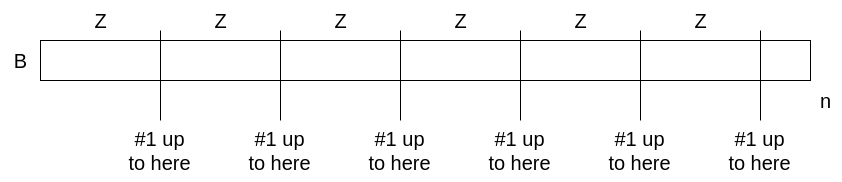
\includegraphics[width=300px]{images/10_Data_compression/rank_select_big_partitions.png}
\end{figure}
Then for each of the big blocks we split them into smaller blocks of $z$ bits and associate to each smaller block the number of 1s from the beginning of the bigger block up to the end of the small block:
\begin{figure}[H]
    \centering
    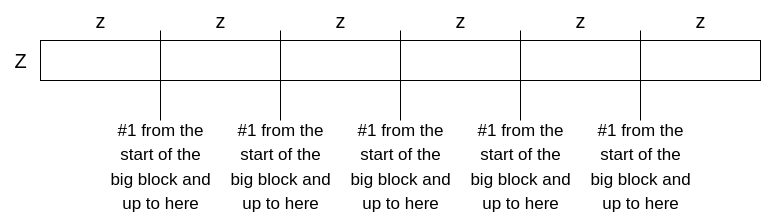
\includegraphics[width=300px]{images/10_Data_compression/rank_select_small_partitions.png}
\end{figure}

So to make a query we need to:
\begin{itemize}
    \item find the big block
    \item find small block
    \item scan for the extra 1s
\end{itemize}

\subsubsection{Space occupancy}
We store $\frac{n}{Z}$ numbers for the big blocks, each number is $log_2 n$ bits so for the bigger blocks we have $\frac{n}{Z} log_2 n$ bits.
Then we need $\frac{n}{z}$ numbers for the smallest blocks each number is $log_2 Z$ bits so the total space occupancy is:
$$
\frac{n}{Z}log_2 n + \frac{n}{z} log_2 Z
$$

If we want to avoid the scan phase we can pre-compute a table with the data for each small block:
\begin{table}[H]
    \centering
    \begin{tabular}{c|c c c c c c}
        conf. of small block | i & 1 & 2 & \_ & i & \_ & z \\
        \hline
        0\_0 &  &  &  &  &  &  \\
        0\_1 &  &  &  &  &  &  \\
        | &  &  &  &  &  &  \\
        0010 & 0 & 0 & 1 & \_ & \_ & \_ \\
        | &  &  &  &  &  &  \\
        1\_1 (z bits) &  &  &  &  &  &  \\
    \end{tabular}
\end{table}
So the table has:
\begin{itemize}
    \item $2^z$ rows;
    \item $z$ cols;
    \item each cell is $\lfloor log_2 z \rfloor$.
\end{itemize}
So total space is:
$$
    \frac{n}{Z}log_2 n + \frac{n}{z}log_2 Z + 2^z \cdot z \cdot log_2 z
$$

Common values for $Z$ and $z$ are:
\begin{itemize}
    \item $Z = log_2^2 n$
    \item $z = \frac{1}{2}log_2 n$
\end{itemize}
Let's substitute:
$$
    \frac{n}{log_2^2n}log_2 n + \frac{n}{\frac{1}{2}log_2 n}log_2 (log_2^2 n) + 2^{\frac{1}{2}log_2 n} \cdot \frac{1}{2}log_2 n \cdot log_2 \left( \frac{1}{2}log_2 n \right) = o(n)
$$

NB: since $z$ is 32 we don't use a table but we just read 32 bits and do a pop count with masks.

NB: now we can state that $\exists$ a rank/select data structure that does not touch $B$, takes $o(|B|) = o(m)$ bits and supports operations in $O(1)$ time, so the total occupancy is:
$$
    |B| + o(|B|) = m + O(m)
$$
Since $n = \#1$ doesn't shows up in the space formula it doesn't depends on n, which means that is useful in the cases in which $B$ is dense!

\subsection{Rank/Select over binary array (sparse version)}
If instead the binary array $B$ is sparse we can use Elias-Fano: we transform $B$ into a sequence of increasing integers and we use the indices of the ones to build our list.
Let's call $A = \{2, 3, 8, 10\}$ the array with the positions of the element to 1 in $B$ and $n = 4$ as the size of that array, we can now encode them with Elias-Fano, so:
\begin{itemize}
    \item $u = 10+1 = 11$;
    \item $b = \lceil log_2 u \rceil = 4$;
    \item $l = \lceil log_2 \frac{u}{n} \rceil = \lceil log_2 \frac{11}{4} \rceil = 2$;
    \item $h = b-l = 4-2 = 2$.
\end{itemize}
let's build the table:
\begin{table}[H]
    \centering
    \begin{tabular}{c | c | c | c}
        x & bin(x) & H(x) & L(x) \\
        \hline
        2 & 0010 & 00 & 10 \\
        3 & 0011 & 00 & 11 \\
        8 & 1000 & 10 & 00 \\
        10 & 1010 & 10 & 10 \\
    \end{tabular}
\end{table}
and build the sequences:
$$
    L = 10110010
$$
$$
    H = 11001100
$$

So now we can use $NextGEQ$ over the sequences L and H if we can implement select operation over H.
To do that we use the other implementation of Rank/Select.
So that we:
\begin{itemize}
    \item $Select_1(x)$ over $B$ is $Access(x)$ over $A$;
    \item $Rank_1(x)$ over $B$ is $NextGEQ(x) -1$ (-1 depends if $x$ is counted in the set or not).
\end{itemize}

\subsubsection{Space occupancy}
L is:
$$
    nlog_2 \frac{u}{n} = nlog_2 \frac{m}{n}
$$
H is:
$$
    2n
$$
In the end the rank/select support over $A$ is $o(n)$, in total:
$$
    nlog_2 \frac{m}{n} + 2n + o(n)
$$
and we get:
\begin{itemize}
    \item select in $O(1)$ time;
    \item rank in $O\left(log_2 \frac{m}{n} \right)$
\end{itemize}

\subsection{Variable-byte code (Altavista)}
We represent $x$ in binary grouping by 7 bits then we pad them (tag each group) to 8 bit using:
\begin{itemize}
    \item 0: if this is the last group for this number;
    \item 1: otherwise
\end{itemize}

NB: if representation in bit is not a multiple of 7 of course you pad it with some 0s.

Using this encoding we use:
$$
    8 \cdot \lceil \frac{|bin(x)|}{7} \rceil \text{ bits}
$$

\subsubsection{Optimal distribution}
If we equalize to $log_2 \frac{1}{p(x)}$ we get the optimal distribution for this encoding which is:
$$
    p(x) = \sqrt[7]{\frac{1}{x^8}} = \frac{1}{x^{\frac{8}{7}}}
$$

\subsubsection{Decoding}
To decode we go byte by byte and if the number is greater than 127 (1-st bit is set) we go on with reading and building the number.


\subsection{(s-c)-dense codes}
In the variable-byte code we have two types of configurations:
\begin{itemize}
    \item \emph{continuers}: configurations of 8 bits that tells us to continue, the one with 1 in front {128, 129, $\_$, 255};
    \item \emph{stoppers}: configurations of 8 bits that tells us to stop, the ones with 0 in front {0, 1, $\_$, 127}.
\end{itemize}
So with this idea in mind we can create a new class of encoding called \emph{(s-c)-dense codes}:
$$
    s + c = 2^b
$$
with:
\begin{itemize}
    \item $s$: the number of stoppers;
    \item $c$: the number of continuers;
    \item $b$: size of the block in bits.
\end{itemize}

Ex: for $b=3$ we can have:
\begin{itemize}
    \item $s = c = 4$;
    \item $s = 6, c = 2$.
\end{itemize}

Of course different combinations of $c$ and $s$ leads to different outcome, for example:
\begin{itemize}
    \item $s=c=4$:
    \begin{itemize}
        \item for single block we can have $s = 4$ different configurations;
        \item for two blocks we can have $s \cdot c = 4^2 = 16$ different configurations;
        \item for three blocks we can have $s \cdot c^2 = 4^3 = 64$ different configurations;
    \end{itemize}
    
    \item $s = 6, c = 2$:
    \begin{itemize}
        \item for single block we can have $s = 6$ different configurations;
        \item for two blocks we can have $s \cdot c = 6 \cdot 2 = 12$ different configurations;
        \item for three blocks we can have $s \cdot c^2 = 6 \cdot 2^2 = 24$ different configurations;
    \end{itemize}
\end{itemize}
In the second configuration if numbers like 4 and 5 are frequent we gain in compression but bits grows faster than the first encoding for larger numbers!

There is an optimal way of partitioning and to choose stoppers and continuers (we won't see those algorithms but are based on dynamic programming).
In general making $c$ bigger helps in encoding more numbers in less bits but making $s$ bigger helps with small numbers.

Ex: encode 8 with a (1-3)-dense code: first we need to check if the exercise is correct, so we need to check if $s+c = 2^b \implies 1+3 = 4 = 2^2 \implies b = 2$ it is correct.
We need to choose the stoppers and the continuers, for example:
\begin{itemize}
    \item 00: stopper;
    \item 01: continuer;
    \item 10: continuer;
    \item 11: continuer.
\end{itemize}
Next we tabulate all the configurations up to 8:
\begin{itemize}
    \item 0: 00;
    \item 1: 01 00;
    \item 2: 10 00;
    \item 3: 11 00;
    \item 4: 01 01 00;
    \item 5: 01 10 00;
    \item 6: 01 11 00;
    \item 7: 10 01 00;
    \item 8: 10 10 00;
\end{itemize}


\subsection{Interpolative coding}
It's an encoding context-aware that exploits patterns in integer sequences, it's very compact as it possibly beats $H_0$ but it's \emph{very} slow!
It use strictly increasing sequences: $S = \{ s_1, s_2, \_, s_n \}$ with $s_i < s_{i+1}$.
It's also a recursive code.

Let's start with some invariants:
\begin{itemize}
    \item $l$: left index;
    \item $r$: right index;
    \item $low$: a lower bound on the values in $S[l, r]$: $low \leq S[i] \forall i \in S[l,r]$;
    \item $high$: an upper bound on the values in $S[l, r]$: $high \geq S[i] \forall i \in S[l,r]$.
\end{itemize}

In encoding phase we start with:
\begin{itemize}
    \item $l = 1$;
    \item $r = n$;
    \item $low = S_1$;
    \item $high = S_n$.
\end{itemize}
we store those values in the preamble of the compressed stream because it's fundamental that compressor and decompressor starts with the same values!

At each phase with $<l, r, low, high>$ we:
\begin{itemize}
    \item $m = \lfloor \frac{l+r}{2} \rfloor$;
    \item we compress $s_m$ given $<l, r, low, high>$ and emit it;
    \item we recursively compress $<l, m-1, low, s_m-1>$;
    \item we recursively compress $<m+1, r, s_m+1, high>$.
\end{itemize}
It's important to notice that in decompression we first decompress $s_m$, then we can use it to derive the new values for the tuple, so the decompressor knows all the values in the tuple or it can calculate them.

Basically we build a structure like:
\begin{figure}[H]
    \centering
    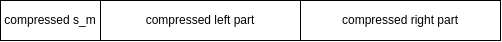
\includegraphics[width=300px]{images/10_Data_compression/interpolative_coding.png}
\end{figure}

\subsubsection{Compress single element}
Since we know that $low \leq s_m \leq high$ we can say:
$$
    0 \leq s_m - low \leq high-low
$$
We would also like to use a fixed size encoding so we need $b = \lceil log_2 (high-low+1) \rceil$ bits.

Ex: $S = \{1, 2, 5, 6, 8, 9, 10\}$, we pick $l=1$, $low=1$, $r = 7$, $high=10$.
Then we calculate $m = 4, s_m = 6$ and we encode $s_m - low = 6-1=5$ in $b = \lceil log_2 (high-low+1) \rceil = \lceil log_2 (10-1+1) \rceil = 4$ bits.
So the final encoded value is $0101$.

Using this encoding we are not exploiting all the informations we have!
If we use also $l$, $r$ and the fact that the sequence is strictly increasing we can calculate another bound for $s_m$: 
$$
    low + (m-l) = low' \leq s_m \leq high' = high - (r-m)
$$
so we can now use $b = \lceil log_2 (high' - low' + 1) \rceil$ bit.

Ex: $S = 4, 5, 6, 7$ leaving the offset they become $0, 1, 2, 3$ so we store 2 bits!

NB: in some contexts we can emit even 0 bits beacuse if we have, for example, 3 elements in the range 7, 8, 9 we know those items and write no bits.

So during the element decompression we need to check if $r-l = high-low$, if that happens simply emit the elements from $high$ to $low$.


\subsubsection{Exercise}
$S = \{ 1, 2, 3, 5, 7, 9, 11, 15, 18, 19, 20, 21 \}$, we pick:
\begin{itemize}
    \item $l = 1$;
    \item $r = 12$;
    \item $low = 1$;
    \item $high = 21$.
\end{itemize}
and we start:
\begin{itemize}
    \item $m = \lfloor \frac{1+12}{2} \rfloor = \lfloor \frac{13}{2} \rfloor = 6$;
    \item $s_m = 9$;
    \item $low' = 1 + (6-1) = 6$;
    \item $high' = 21 - (12-6) = 15$;
    \item new range: $6 \leq 9 \leq 15$;
    \item shifted range: $0 \leq 3 \leq 9$;
    \item $b = \lceil log_2 (15-6+1) \rceil = 4$;
    \item we emit $0011$; (3 over 4 bits).
\end{itemize}

The left recursive call uses $<1, 5, 1, 8>$ and the right recursive call uses $<7, 12, 10, 21>$.


\subsection{Pointerless programming}
Let's implement a binary (search) tree without pointers: let's transform  the one in the figure.
\begin{figure}[H]
    \centering
    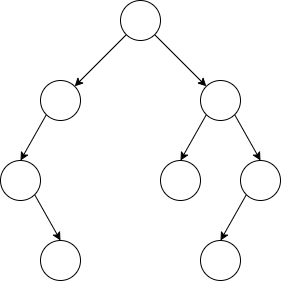
\includegraphics[width=150px]{images/10_Data_compression/pointerless_programming_start.png}
\end{figure}
To make it pointerless we need to apply some transformations.

First we \emph{complete the tree}: we fill the tree so that each node is fully binary (each node has two sons):
\begin{figure}[H]
    \centering
    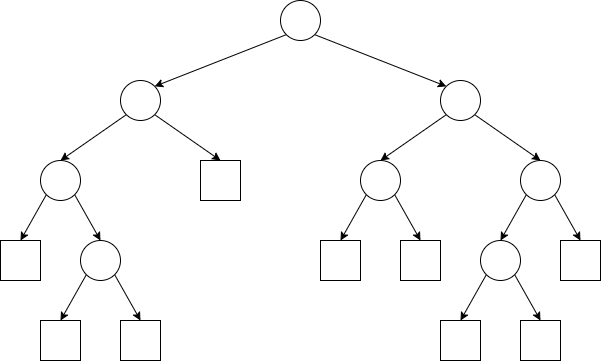
\includegraphics[width=250px]{images/10_Data_compression/poitnerless_programming_complete.png}
\end{figure}

Then we visit the completed tree in a BFS way and we label each node from 1 to $2n-1$ and also mark the actual real nodes with another incremental counter:
\begin{figure}[H]
    \centering
    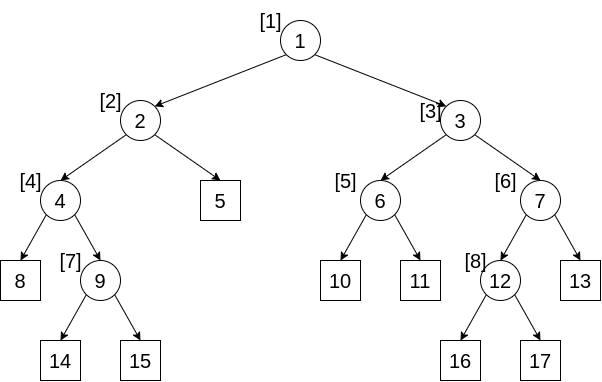
\includegraphics[width=250px]{images/10_Data_compression/pointerless_labeled.png}
\end{figure}

In the end we serialize the structure, to do it we execute another BFS and create a bitvector with 1 in corrispondence of the existing nodes and 0 otherwise:
$$
    B = 11110110100100000
$$
then we build a Rank/Select support over $B$ (using the first implementation), so the space occupancy is:
$$
 |B| + o(|B|) = 2n + 1 + o(n)
$$
So we use 2 bits per node instead of 128 using two pointers for the sons.

\subsubsection{Navigate the tree}
The labeling is similar to the one we use inside an heap but this is not completely the case since the tree is not actual like heap, in particular we use:
\begin{itemize}
    \item $left([x]) = 2x$;
    \item $right([x]) = 2x + 1$.
\end{itemize}
So the navigation is from the real node number to the completed tree number.
To check if the node exists we just need to check in $B$ if the bit in the corresponding plain position is set to 1:
\begin{itemize}
    \item left child exists iff $B[2x] = 1$;
    \item right child exists iff $B[2x+1] = 1$.
\end{itemize}

To translate from plain number to tagged one we use $Rank(x)$:
\begin{itemize}
    \item to access to the left child of $[x]$ we access to the index returned by $Rank_1(2x)$;
    \item to access to the right child of $[x]$ we access to the index returned by $Rank_1(2x+1)$.
\end{itemize}

To go up to the parent we do the reverse:
$$
    parent([x]) = \lceil \frac{Select_1(x)}{2} \rceil
$$

\subsubsection{Store information}
Of course we want to add some information to the nodes of the tree so we store aside from the tree an array in which we use the tagged index from the tree to access the actual element associated to that node.

\subsubsection{Exercise}
Check if path $\pi[1, p]$ exists starting from the root.
% TODO

\section{Data Compression}
\subsection{Statistical compressor}
Let's call $\Sigma$ the alphabet, it can be made from different types of data:
\begin{itemize}
    \item letters, so we have at most 26 objects;
    \item words, so we have something $O(millions)$;
    \item integers, so thery are virtually infinite;
    \item bytes, so we have 256 objects;
    \item ...
\end{itemize}

So depending on the alphabet we change the store and the alphabet size. Since the decompressor must know the alphabet we build a structure before the stream of compressed data, called \emph{preamble} which contains the alphabet representation, the frequencies of the symbols and other informations.

\subsection{Huffman Encoding}
Huffman encoding is a greedy algorithm which gets the optimal encoding for it's class.
It builds a tree exploiting the frequencies of the symbols.

Let's assume we have $\Sigma=\{a, b, c, d, e, f\}$ and the frequencies are:
\begin{itemize}
    \item $a$: 0.05;
    \item $b$: 0.1;
    \item $c$: 0.15;
    \item $d$: 0.3;
    \item $e$: 0.25;
    \item $f$: 0.15.
\end{itemize}

We need to build a tree so we start with just the leaves, one for each symbol:
\begin{figure}[H]
    \centering
    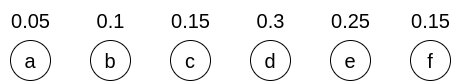
\includegraphics[width=200px]{images/10_Data_compression/huffman_0.png}
    \caption{Step 0}
\end{figure}
and we build it joining the two nodes with the lowest frequencies in a single node with frequency equals to the sum of the two single nodes:
\begin{figure}[H]
    \centering
    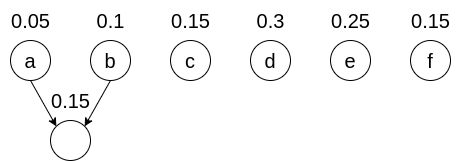
\includegraphics[width=200px]{images/10_Data_compression/huffman_1.png}
    \caption{Step 1}
\end{figure}
And we go on in the same way at each round:
\begin{figure}[H]
    \centering
    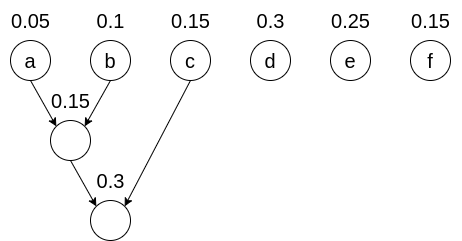
\includegraphics[width=200px]{images/10_Data_compression/huffman_2.png}
    \caption{Step 2}
\end{figure}

In the end we get a complete binary tree:
\begin{figure}[H]
    \centering
    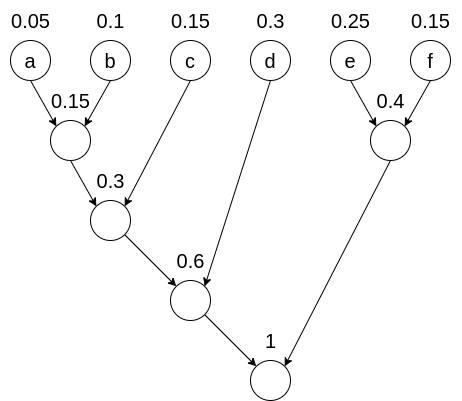
\includegraphics[width=200px]{images/10_Data_compression/huffman_5.png}
    \caption{Final step}
\end{figure}

Since it is binary we have $\sigma = |\Sigma|$ leaves, one for each symbol.

To assign an encoding we can:
\begin{itemize}
    \item assign 0 to each left branch;
    \item assign 1 to each right branch
\end{itemize}
and the symbol encoding is just the path to reach it:
\begin{figure}[H]
    \centering
    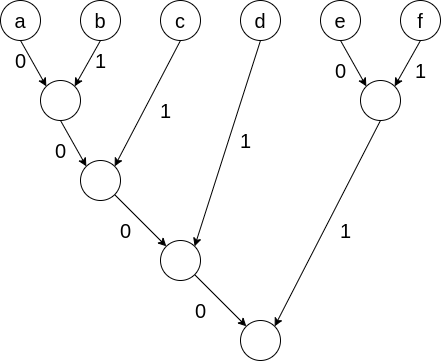
\includegraphics[width=200px]{images/10_Data_compression/huffman_encoding.png}
\end{figure}

So in this case we have the following encoding:
\begin{itemize}
    \item a: 0000;
    \item b: 0001;
    \item c: 001;
    \item d: 01;
    \item e: 10;
    \item f: 11.
\end{itemize}
It's important to notice that we gain a prefix-free code!

We have $s^{\sigma-1}$ different labeling ways.

NB: whenever we can make different choices to merge nodes it is better to merge the oldest nodes, that minimizes the maximum code-word length. (But the code is always optimal regardless the maximum length!)

To decode a sequence of bits we just need to traverse the tree until we reach a leaf, and that leaf is the encoded character.

\subsubsection{Optimality}
The average code-word length is:
$$
    L_c = \sum_{s \in \Sigma} p(s) \cdot |cw(s)|
$$
but it is equivalent to the average depth of a leaf.

The key property of this algorithm is that \emph{Huffman code is optimal among all prefix-free codes}, let's prove it.

Lemma 1: let $F$ be the set of binary trees whose average depth is minimum over the binary trees with $\sigma$ leaves, then $\exists T \in F$ such that the two leaves of smallest $\mathbb{P}$ are at the largest depth and they are children of the same parent:
\begin{figure}[H]
    \centering
    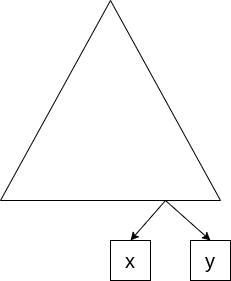
\includegraphics[width=100px]{images/10_Data_compression/huffman_proof_1.png}
    \caption{$x, y$ have the smallest $\mathbb{P}$}
\end{figure}
Let's prove the lemma by contraddiction: let's build a tree in which the leaves with the smallest probability are not at the end of the tree:
\begin{figure}[H]
    \centering
    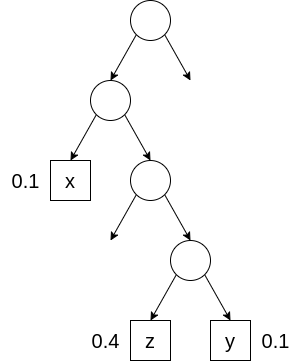
\includegraphics[width=200px]{images/10_Data_compression/huffman_contraddiction.png}
\end{figure}
Let's check the average depth:
$$
    0.1 \cdot 3 + 0.4 \cdot 5 + 0.1 \cdot 5 + \_
$$
this tree should have the minimum avg depth but if we swap $x$ with $z$ we get:
$$
    0.4 \cdot 3 + 0.1 \cdot 5 + 0.1 \cdot 5 + \_
$$
which for sure is smaller!

Lemma 2: we will study the following reduction in which we join he probability of two leaves into a single node:
\begin{figure}[H]
    \centering
    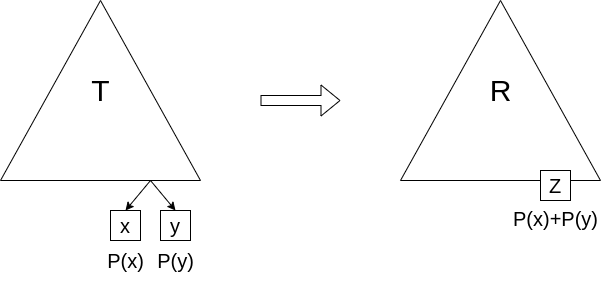
\includegraphics[width=300px]{images/10_Data_compression/huffman_lemma_2.png}
\end{figure}
We want to know the relation between average depth of both the trees:
$$
    L_T = \sum_{\text{s leaves}} depth(s) \cdot \mathbb{P}(s)
$$
$$
    = \sum_{\text{s leaves} \neq x,y} depth(s) \cdot \mathbb{P}(s) + depth(x) \cdot \mathbb{P}(x) + depth(y) \cdot \mathbb{P}(y)
$$

$$
    L_R = \sum_{\text{s leaves}} depth(s) \cdot \mathbb{P}(s)
$$
$$
    = \sum_{\text{s leaves} \neq z} depth(s) \cdot \mathbb{P}(s) + depth(z) \cdot (\mathbb{P}(x) + \mathbb{P}(y))
$$
so let's study the difference:
$$
    L_T - L_R = depth(x) \cdot \mathbb{P}(x) + depth(y) \cdot \mathbb{P}(y) - depth(z) \cdot \mathbb{P}(z) =
$$
let's call $l = depth(z)$:
$$
    = (l+1)(\mathbb{P}(x)+\mathbb{P}(y)) - l\cdot(\mathbb{P}(x)+\mathbb{P}(y)) = 
$$
$$
    = (l+1 - l)(\mathbb{P}(x)+\mathbb{P}(y)) = 
$$
$$
    = p(x)+p(y) 
$$
So we can write: $L_T = L_R + \mathbb{P}(x) + \mathbb{P}(y)$

Let's prove that average depth of Huffman tree is minimum: let's call $L_H$ the tree obtained from Huffman encoding algorithm, then we want to prove that $L_H <= L_T \forall T $ with $\sigma$ leaves.
By induction:
\begin{itemize}
    \item case with $\sigma = 2$: there is only one way to build a tree so it is an Huffman tree and since the only one, it is optimal;

    \item by induction we impose that Huffman with $\sigma-1$ symbols is optimal so let's prove that it's true for $\sigma$ symbols too: by contraddiction let $C$ be an optimal tree that satisfies lemma 1, then $L_C$ is the average depth of $C$, so we apply the Lemma 2 obtaining $Rc$, now we can say:
    $$
        L_C = L_{Rc} + \mathbb{P}(x) + \mathbb{P}(y)
    $$
    $Rc$ has $\sigma-1$ leaves s we can apply the inductive hypothesis so there exists an Huffman tree with $\sigma-1$ leaves that is optimal, let's call it $H$, now we have:
    $$
        L_{Rc} \geq L_H
    $$
    and:
    $$
        L_C = L_{Rc} + \mathbb{P}(x) + \mathbb{P}(y) \geq L_H + \mathbb{P}(x) + \mathbb{P}(y)
    $$
    So now we take $H$ which has a leaf with probability $\mathbb{P}(x) + \mathbb{P}(y)$ and split it in two more leaves.
    The new tree is an Huffman tree because the rest of the tree is an Huffman tree and $\mathbb{P}(x)$ and $\mathbb{P}(y)$ are least probable leaves, let's call it $E_H$ (enlarged), for Lemma 2 we have:
    $$
        L_{Eh} = L_{H} + \mathbb{P}(x) + \mathbb{P}(y) \leq L_C
    $$
    so the Huffman tree obtained, with $\sigma$ leaves, is optimal!
\end{itemize}

\subsubsection{Performance}
It can be proved that:
$$
    H \leq L_{Huffman} < H+1
$$
in which:
\begin{itemize}
    \item $H$: is the entropy of the source;
    \item $L_{Huffman}$: is the average code-word length in bits.
\end{itemize}

But of course the problem is $H: 0 \leq H \leq log_2 \sigma$, so:
\begin{itemize}
    \item if $H=20$, 1 bit means nothing;
    \item if $H=2$, 1 bit is a lot.
\end{itemize}
So it is optimal for random sources but awful for repetitive ones.

\subsubsection{One note}
$$
    L_H = \sum_{s \in \Sigma}\mathbb{P}(s) \cdot |cw(s)|
$$
with $|cw(s)| \in \mathbb{N}$,
$$
    H = \sum_{s \in \Sigma}\mathbb{P}(s) \cdot log_2 \frac{1}{\mathbb{P}(s)}
$$
with $log_2 \frac{1}{\mathbb{P}(s)} \in \mathbb{R}$.
So it could be $H < L_H$ but still be optimal!
To avoid fractional bits we can pack many symbols together to spread the additional bit among more symbols!

\subsection{Canonical Huffman}
An Huffman tree in canonical form is a tree formed in the following way:
\begin{figure}[H]
    \centering
    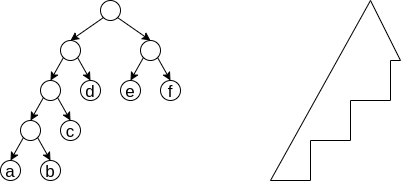
\includegraphics[width=300px]{images/10_Data_compression/canonical_huffman.png}
\end{figure}
and it can be stored without the use of any pointer thus speeding up a lot the decompression!

It is faster also because we can encode the first code-word of each level and then derive the other ones from the first one, so we also make the preamble smaller.

Let's call them \emph{first code-word} ($f_c$):
\begin{itemize}
    \item $a$: 0000 $ = f_c[4]$;
    \item $c$: 001 $ = f_c[3]$;
    \item $d$: 01 $ = f_c[2]$.
\end{itemize}

So given a code-word the next ones can be obtained just increasing.
Of course we need the size of the level bu we can store just the $f_c$ array and a symbol table:
\begin{itemize}
    \item $f_c[4] = $ 0000;
    \item $f_c[3] = $ 001;
    \item $f_c[2] = $ 01;
    \item $f_c[1] = $ ?.
\end{itemize}

\begin{table}[H]
    \centering
    \begin{tabular}{c|c c c}
        index & symbols \\
        \hline
        1 & // & & \\
        2 & d & e & f \\
        3 & c & & \\
        4 & a & b & \\
    \end{tabular}
\end{table}

Using the canonical tree we can check if a bit combination exists on a certain level just checking if we are on the left or on the right of the first code-word of that level.

For the levels with no code-words we store in $f_c$ an element which can't be on that level, greater than everyone else, for example $f_c[1] = 10$ which is surely bigger than $1$ and $0$ which are the only code-words that can be used on level 1.

The pseudo-code to decode a symbol is:
\begin{verbatim}
    DecodeSymbol()
        v = next_bit()
        l = 1
        
        while (v < fc[l])
            v = 2*c + next_bit()
            l++
        return symbol[l][v-fc[l]]
\end{verbatim}

NB: we could have a cache miss in symbol table access but if symbols aren't too much we can fit entire table in cache.

\subsubsection{Build canonical form}
To build a canonical Huffman tree we:
\begin{itemize}
    \item construct the Huffman tree;
    \item compute the array $num[1, l]$ s.t. $num[i] = \#$symbols at level $i$ in Huffman tree;
    \item compute symbol table;
    \item compute first code-word array s.t.:
    \begin{equation}
        \begin{cases}
            f_c[l] = 0 \\
            f_c[i] = \frac{f_c[i+1] + num[i+1]}{2}
        \end{cases}
    \end{equation}
\end{itemize}

Once the tree is built we build metadata and then dump the tree.

\subsubsection{Encoding algorithm}
To encode a symbol we:
\begin{itemize}
    \item search for the symbol in the symbol table, get $l$ and $offset$;
    \item the encoding is $f_c[l] + offset$ in $l$ bits.
\end{itemize}

\subsection{Arithmetic encoding}
It's and encoding which exploits the floating point representation of numbers to map a sequence to a number in the range $[0, 1)$.
Of course it is a statistical method so we need to know the frequencies/probabilities for each symbol.

\subsubsection{Floating point numbers}
Given $x \in [0, 1)$ we can represent it with:
$$
    x = 0.b_1b_2b_3\_b_k\_
$$
It is a positional representation because each bit represent $\frac{1}{2^k}$ and $b_i \in \{0, 1\}$.

For example: $0.101_2 = \frac{1}{2} + \frac{1}{8} = \frac{5}{8}$.
The number in the form:
$$
    \frac{v}{2^a}
$$
with:
\begin{itemize}
    \item $v$: the representation of the fractional part of the numbers;
    \item $a$: the number of bits of the fractional part.
\end{itemize}
are called \emph{dyadic fractions}.
Ex:
$$
    0.1011_2 = \frac{11}{16}
$$
and $1011_2 = 11$ on $4$ digits $2^4 = 16$.

We can make a function to convert any number in this binary representation:
\begin{verbatim}
    Converter(x, k)
        for i in 0..k:
            if 2x < 1:
                emit 0
                x = 2x
            else
                emit 1
                x = 2x - 1
\end{verbatim}
This algorithms create the number from left to right so we can stop whenever we want.

Given $x \in [0,1)$ if we truncate $x$ to the first $d$ bits we get $\tilde{x}$ and we can state that:
$$
    0 \leq x-\tilde{x} \leq 2^{-d}
$$

We can visually prove it:
\begin{table}[H]
    \centering
    \begin{tabular}{c c c c c c | c c c}
        $x $ & $.b_1$ & $b_2$ & $b_3$ & $\_$ & $b_d$ & $b_{d+1}$ & $b_{d+2}$ & $\_$ \\
        $\tilde{x} $ & $.b_1$ & $b_2$ & $b_3$ & $\_$ & $b_d$ & $0$ & $0$ & $\_$ \\
        $x-\tilde{x} $ & $0$ & $0$ & $0$ & $\_$ & $0$ & $b_{d+1}$ & $b_{d+2}$ & $\_$ \\
    \end{tabular}
\end{table}
so for sure the result has $d$ leading zeroes:
$$
    x-\tilde{x} = \sum_{i=d+1}^\infty b_i \cdot 2^{-i} = \sum_{i=1}^\infty b_{d+1} \cdot 2^{-(d+i)} \leq \sum_{i=1}^\infty 2^{-(d+i)} = 
$$
$$
    = 2^{-d} \sum_{i=1}^\infty 2^{-i} = 2^{-d}
$$

\subsubsection{Encoding}
Starting from the frequencies of each symbol:
\begin{itemize}
    \item $\mathbb{P}(a) = \frac{1}{2}$;
    \item $\mathbb{P}(b) = \frac{1}{4}$;
    \item $\mathbb{P}(c) = \frac{1}{4}$.
\end{itemize}
we compute the cumulative frequency:
\begin{itemize}
    \item $f_a = 0$;
    \item $f_b = p(a) = \frac{1}{2}$;
    \item $f_c = p(a) + p(b) = \frac{3}{4}$.
\end{itemize}

Then starting with the interval $[0, 1)$ we split it according to the probability of each symbol:
\begin{figure}[H]
    \centering
    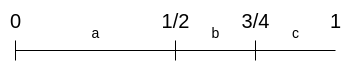
\includegraphics[width=225px]{images/10_Data_compression/arithmetic_encoding_0.png}
\end{figure}

Then looping over each symbol of the sequence we focus on the interval specified by the symbol, for example $S = a, b, a, c$:
\begin{figure}[H]
    \centering
    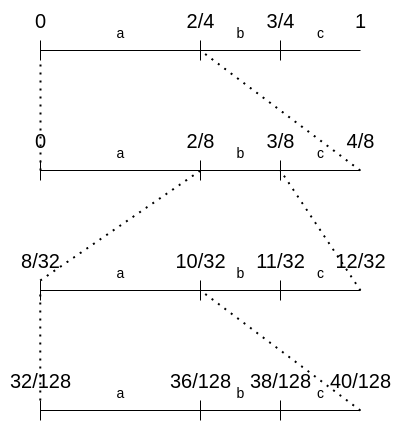
\includegraphics[width=225px]{images/10_Data_compression/arithmetic_encoding_1.png}
\end{figure}

Formally we use two numbers to remember the range and navigate it:
\begin{itemize}
    \item $l$: left interval;
    \item $s$: size of the interval.
\end{itemize}
we start with:
\begin{itemize}
    \item $l=0$;
    \item $s=1$
\end{itemize}
and at each iteration we update the values according to:
\begin{itemize}
    \item $l_i = l_{i-1} + s_{i-1} \cdot f(T[i]) $
    \item $s_i = s_{i-1} \cdot \mathbb{P}(T[i])$
\end{itemize}

Once we are over with the navigation we compute:
$$
    x = l + \frac{s}{2}
$$
so basically we compute the middle element inside the range.
We don't actually need exactly the element in the middle but any number which lays in the range so we can truncate the representation to the minimum number inside the range: $\tilde{x} = $ truncation of $x$ at $d$ bits with:
$$
    d = \lceil log_2 \frac{2}{s} \rceil \leq 2^{-d}
$$

Let's prove that $\tilde{x}$ is in the range:
$$
    2^{-d} = 2 ^{-\lceil log_2 \frac{2}{s} \rceil} = \frac{1}{ 2 ^{\lceil log_2 \frac{2}{s} \rceil} } \leq \frac{1}{ 2 ^{log_2 \frac{2}{s}} } = \frac{1}{\frac{2}{s}} = \frac{s}{2}
$$

The size changes according to the probability of the symbols:
\begin{itemize}
    \item $s_0 = 1$;
    \item $s_1 = \mathbb{P}(a)$;
    \item $s_2 = s_1 \cdot \mathbb{P}(b) = \mathbb{P}(a) \cdot \mathbb{P}(b) $;
    \item $s_2 = s_2 \cdot \mathbb{P}(a) = \mathbb{P}(a) \cdot \mathbb{P}(b) \cdot \mathbb{P}(a) $;
\end{itemize}

\subsubsection{Decoding}
We interpret the resulting sequence as a floating point number and check where it lays in those partitions, once we get the partition we get the letter and move on to the next partitioning.

NB: we can compress how many symbols we want so during the decompression we need to know how many symbols we need to decompress!

\subsubsection{Performance}
$$
    d = \lceil log_2 \frac{2}{s} \rceil = \lceil 1 + log_2 \frac{1}{s} \rceil = \lceil 1 - log_2 s \rceil < 2 - log_2 s
$$
since: $s = \mathbb{P}(a) \cdot \mathbb{P}(b) \cdot \mathbb{P}(a) \cdot \mathbb{P}(c)$ we can say:
$$
    d < 2 - log_2 \prod_{i=1}^n \mathbb{P}(T[i]) = 2 - \sum_{i-1}^n log_2 \mathbb{P}(T[i])
$$

NB: 
$$
    \sum_{i-1}^n log_2 \mathbb{P}(T[i]) = log_2 \mathbb{P}(a) + log_2 \mathbb{P}(b) + log_2 \mathbb{P}(a) + log_2 \mathbb{P}(c) = 
$$
$$
    = 2log_2 \mathbb{P}(a) + log_2 \mathbb{P}(b) + log_2 \mathbb{P}(c) = 
$$
so we have the frequency of a symbol times the logarithm of the probability of the symbol, so:
$$
    = 2 - \sum_{\sigma} occ(\sigma) \cdot log_2 \mathbb{P}(\sigma) = 2 + \sum_{\sigma} occ(\sigma) \cdot log_2 \frac{1}{\mathbb{P}(\sigma)} = 
$$
$$
    = 2 + n \cdot \sum_{\sigma} \frac{occ(\sigma)}{n} \cdot log_2 \frac{1}{\mathbb{P}(\sigma)} = 2 + n \cdot \sum_{\sigma} \mathbb{P}(\sigma) \cdot log_2 \frac{1}{\mathbb{P}(\sigma)}
$$
$$
 = 2 + nH
$$

So the total number emitted for all the text is $2 + nH$, then the average bits emitted per symbol is:
$$
\frac{d}{n} \leq \frac{nH + 2}{n} = H + \frac{2}{n}
$$

The longer the text, the more we are converging to the entropy!
But we are assuming infinite size floating point number which is not the case in practice.
In the application we get something like $H + \frac{1}{100}$ on fixed size text blocks.

\subsection{Dictionary-based compressors}
Up to now we have seen statistical compressor/coders, which uses frequencies.
Now we'll see some dictionary-based compressors which uses syntactic.
In particular we'll see the ones from Lempel and Ziv: LZ77 and LZ78 which are the bases of \emph{gzip}, \emph{Brotli}, \emph{ZSTD} and \emph{LZFSE}.

\subsection{LZ77}
Let's consider the followind sequence:
$$
    T = aacaacabcaaaaaaac
$$
and suppose that you've already processed up to $aacaacab$, so we want to encode the next part, we can \emph{copy} the next part $caa$ from before and append an \emph{extra} character $a$.
So we need to build a dictionary of all substrings starting before the current point.
Of course we can't store all the dictionary D.

To compress we search for the biggest prefix string for the string we want to compress, we call that part \emph{copy} and the new character \emph{extra}.
So for each sequence we compress we emit a tuple of the type:
$$
    <distance, length, extra>
$$
with:
\begin{itemize}
    \item distance: the distance from the current mark to the start of the copy section;
    \item length: size of the copy section;
    \item extra: extra character to add once copied.
\end{itemize}

So in that case we would emit: $<6, 3, a>$.

NB: suppose we need to compress the sequence $aaaaac$ and we've already compressed the first character with $<0, 0, a>$ we can compress the following part with just $<1, 4, c>$.
Since we copy using the following algorithm:
\begin{verbatim}
    for(i=0; i < l; i++)
        T[cursor+i] = T[cursor-d+i]
\end{verbatim}
we can also exploit overlapping sequences.
An overlap can be detected checking if $l > d$.

NB: this compression in the worst case can grow in size the input data so it is important to compress on a buffer with 1.2 times the initial size.

\subsubsection{LZSS}
An improved version of LZ77 is LZSS.
At the start of LZ77 we copy nothing so the emitted symbol is $<0, 0, a>$, we can exploit it and emitting two types of symbols:
\begin{itemize}
    \item $<0, d>$: if the first element is 0 we don't copy and add a character;
    \item $<d, l>$: if the first element is not 0 we copy using $d$ and $l$ just like before.
\end{itemize}

\subsubsection{Full example}
$$
    T = aacaacabcaaaaaaac
$$
Using LZ77:
\begin{itemize}
    \item $a$ emits: $<0, 0, a>$;
    \item $ac$ emits: $<1, 1, c>$;
    \item $aacab$ emits: $<3, 4, b>$;
    \item $caaa$ emits $<6, 3, a>$;
    \item $aaaac$ emits: $<1, 4, c>$.
\end{itemize}
To store the tuples we can build some lists:
$$
    T_d = \{0, 1, 3, 6, 1\} \\
    T_l = \{0, 1, 4, 3, 4\} \\
    T_c = \{a, c, b, a, c\}
$$
and then we compress each list using Huffman exploiting the even distribution of the symbols.

Using LZSS:
\begin{itemize}
    \item $a$ emits: $<0, a>$;
    \item $ac$ emits: $<1, 1>$;
    \item $aaca$ emits: $<3, 4>$;
    \item $b$ emits: $<0, b>$;
    \item $caa$ emits: $<6, 3>$;
    \item $aaaaa$ emits: $<2, 5>$;
    \item $c$ emits: $<8, 1>$;
\end{itemize}

\subsubsection{Speed up the algorithm}
To speed up the algorithm we introduce a \emph{window} which is the maximum distance we can check for whenever we scan back.
In \emph{gzip} we can specify as a parameter: -1, -2, $\_$, -9 which means the window size in kilobytes.

To find prefixes faster we can use an hash-table of triples of chars:
\begin{itemize}
    \item $<aac, 1>$;
    \item $<aca, 2>$;
    \item $<\_, \_>$
\end{itemize}
so if the window is of size $w$ we will have $w$ items in the hash-table.

To compute a match we take a triple, search in the hash-table, we take all the matches and we brute-force the longest match among the ones we have.
If there is no match we advance by one character.

We can update the hash-table deleting the triples outside of the window while we advance it and just pushing the new ones.
To do it faster we can add pointers to hash-table entries to link each triple to the next one in order, so with just an head and a tail we can delete elements without searching in the hash-table.

\subsection{LZ78}
This time we build up a real dictionary $D$:
$$
    T = aabaacabcabcb
$$
Initially the dictionary is empty so processing $a$ and searching for the longest copy in $D$ we get the empty string, so we emit the tuple $<0, a>$ in which the first number is the number of the entry in the dictionary and the character is the \emph{extra} to append.
Then we update the dictionary.

Then we go for $a$, there is a match inside the dictionary so we go for $ab$, no match so we emit $<1, b>$ and add this entry to the dictionary.

Then we go for $a$, there is a match, so we go for $aa$, no match so we emit $<1, a>$ and add this entry to the dictionary.

We build the dictionary using a trie since we are looking for prefixes, in the end we will build something like:
\begin{figure}[H]
    \centering
    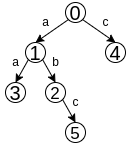
\includegraphics[width=100px]{images/10_Data_compression/LZ78_dictionary.png}
\end{figure}

Of course the trie grows a lot so at certain point we can freeze the dictionary  or discard it and start again from scratch.

\subsubsection{Decode}
To decode we just need to build the trie again and decode each tuple.
To find the node faster in the trie we can keep an array of pointers to the nodes and traverse the tree upward.

\subsection{Some stats}
\subsubsection{Compression ratio}
Compression ratio is defined as:
$$
    \frac{\text{size compressed}}{\text{original size}}
$$
so the smaller the better.

\subsubsection{Compression speed}
$$
    \frac{\text{original size}}{\text{time to compress}}
$$

\subsubsection{Decompression speed}
$$
    \frac{\text{original size}}{\text{time to decompress}}
$$

\subsection{Burrows-Wheeler transform}
This algorithm is the base for the bzip2 command on linux.
It's called block sorting compressor and in general it splits data in blocks, each block then is compressed (applying some transformations) and we do some sort inside the block.
But we need some tools before.

\subsubsection{Move To Front (MTF)}
It's a transformation from symbols to symbols that tries to exploit local homogeneity.
Let's use the sequence $T = abaabacdccddd$, we transform it to a sequence of small integers:
\begin{itemize}
    \item we take the alphabet $\Sigma = \{a, b, c, d\}$;
    \item we start creating new sequence $S^{MTF}$ using list $l = (a, b, c, d)$.
    Substituting each symbol in $T$ with its position in $l$, then we move that position to the front of $l$.
\end{itemize}

Ex:
\begin{itemize}
    \item emit $0$, push $a$ in front, $l=(a, b, c, d)$;
    \item emit $1$, push $b$ in front, $l=(b, a, c, d)$;
    \item emit $1$, push $a$ in front, $l=(a, b, c, d)$;
    \item emit $0$, push $a$ in front, $l=(a, b, c, d)$;
    \item emit $1$, push $b$ in front, $l=(b, a, c, d)$;
    \item emit $1$, push $a$ in front, $l=(a, b, c, d)$;
    \item emit $2$, push $c$ in front, $l=(c, a, b, d)$;
    \item emit $3$, push $d$ in front, $l=(d, c, a, b)$;
    \item emit $1$, push $c$ in front, $l=(c, d, a, b)$;
    \item emit $0$, push $c$ in front, $l=(c, d, a, b)$;
    \item emit $1$, push $d$ in front, $l=(d, c, a, b)$;
    \item emit $0$, push $d$ in front, $l=(d, c, a, b)$;
    \item emit $0$, push $d$ in front, $l=(d, c, a, b)$;
\end{itemize}
Using this MTF we can exploit local homogeneity since we use same symbols and sometimes we change context (for example we have 2-3 when we switch from $ab$ to $cd$).

NB: let's suppose we have this string:
$$
    X = 1^n 2^n 3^n \_ n^n \\
    |X| = n^2
$$
for $n$ different numbers.
Using Huffman we would have:
$$
    \mathbb{P}(1) = \mathbb{P}(2) = \_ = \mathbb{P}(n) = \frac{1}{n}
$$
so $|cw(1)| = |cw(2)| = \_ = |cw(n)| = log_2 n$ bits, so we would produce $|X|log_2 n = n^2log_2 n$ bits.
Suppose now to pass the sequence $X$ via MTF and encode the result with $\gamma$-code:
$$
    MTF(x) = ?000\_0?000\_0\_?000\_0
$$
each block would be formed by:
\begin{itemize}
    \item one number which indicates the actual position of the new character in $l$;
    \item $n-1$ zeroes because now the element is on the first position of $l$.
\end{itemize}
The $\gamma$-encode (note that $\gamma$-code start from 1, so we shift each number, so we encode $x+1$) is:
$$
    \gamma(MTF(X)) = ?111\_1?111\_1\_?111\_1
$$
in which each block is formed by:
\begin{itemize}
    \item a starting which is at most $|\gamma(n)| \leq O(log_2 n)$ bits;
    \item $n-1$ bits to 1 to encode the zeroes.
\end{itemize}
So the whole sequence is at most:
$$
    O(n \cdot log_2 n)  + n(n-1)
$$
so we have $O(n^2)$ bits instead of the $O(n^2log_2 n)$ bits with Huffman.
That's because Huffman is a prefix-free code in which we assign the same code to each symbol.
But in the new encoding we don't use prefix-free codes!

\subsubsection{Run-Length Encoding (RLE)}
Let's suppose here too to have the sequence:
$$
    a^n b^n c^n \_
$$
and we encode it with the tuples: $<a, n>, <b, n>, <c, n>, \_$.
For each run of equal symbols we emit a couple.
It is good when local homogeneity property is strong!

NB: It was used in FAX machines: suppose we have two lines:
$$
    01101000111 \\
    01000000110
$$
we xor them obtaining $00101000001$ and we encode it with $0, 2, 1, 1, 1, 5, 1$ in which the first symbol says the starting bit, then each number says the size of each run, then it is encoded with Huffman.

\subsubsection{Bzip}
The algorithm is the following:
\begin{itemize}
    \item rotate the text and make all the rotating permutations;
    \item sort the strings;
    \item take the last row and call it $L$ (we take the last character of each permutation after sorting them);
    \item move to front code the string $L$;
    \item run-length the resulting sequence;
    \item apply statistical coder.
\end{itemize}

To come back from $L$ to the original string we need some observations:
\begin{itemize}
    \item we can compute the first column ($F$) of the matrix just by sorting $L$;
    \item each row of the matrix is a suffix of the original string;
    \item having $F$ and $L$ we can compute couples of near characters;
    \item all the occurrences of a same symbol $c$ in $L$ maintain the same order as in $F$.
\end{itemize}
Using all the properties described above (in particular the last one) we can rebuild the original string backward starting from the end symbol $\$$ which will be the the first row.

Example with the string $mississipi\$$:
\begin{itemize}
    \item let's build the matrix with all the permutations:
    \begin{verbatim}
        mississipi$
        ississipi$m
        ssissipi$mi
        sissipi$mis
        issipi$miss
        ssipi$missi
        sipi$missis
        ipi$mississ
        pi$mississi
        i$mississip
        $mississipi
    \end{verbatim}

    \item we sort them:
    \begin{verbatim}
        $mississipi        
        ississipi$m
        issipi$miss
        ipi$mississ
        i$mississip
        mississipi$
        pi$mississi
        ssissipi$mi
        sissipi$mis
        ssipi$missi
        sipi$missis
    \end{verbatim}

    \item take $L = imssp\$iisis$.
\end{itemize}

To decode we start with $L = imssp\$iisis$ and:
\begin{itemize}
    \item we compute $F$ by sorting $L$, so: $F = \$iiiimpssss$;
    \item we build the string backwards starting from $\$$:
    \begin{itemize}
        \item character before $\$$ is $i$;
        \item last appearance of $i$ in $F$ is on row 5, so the character before is $p$;
        \item last appearance of $p$ in $F$ is on row 7, so the character before is $i$;
        \item third appearance of $i$ in $F$ is on row 4, so the character before is $s$;
        \item last appearance of $s$ in $F$ is on row 11, so the character before is $s$;
        \item third appearance of $s$ in $F$ is on row 10, so the character before is $i$;
        \item second appearance of $i$ in $F$ is on row 3, so the character before is $s$;
        \item second appearance of $s$ in $F$ is on row 9, so the character before is $s$;
        \item first appearance of $s$ in $F$ is on row 8, so the character before is $i$;
        \item first appearance of $i$ in $F$ is on row 2, so the character before is $m$
    \end{itemize}
\end{itemize}
so the recovered string is $mississipi\$$.

\subsubsection{Full example}
Given $L = abrbb\$aa$, we encode it in $<abrbbaa, 5>$ in which the second number says the position of the end of string.
We apply MTF:
\begin{itemize}
    \item $l=(a, b, r)$, $a -> 0$;
    \item $l=(a, b, r)$, $b -> 1$;
    \item $l=(b, a, r)$, $r -> 2$;
    \item $l=(r, b, a)$, $b -> 1$;
    \item $l=(b, r, a)$, $b -> 0$;
    \item $l=(b, r, a)$, $a -> 2$;
    \item $l=(a, b, r)$, $a -> 0$;
\end{itemize}
so $MTF(X) = <<0, 1, 2, 1, 0, 2, 0>, <a, b, r>, 5> $

The RLE is done only on runs of zeroes: for example $X = 1, 0, 0, 0, 0, 2, 0, 0, 0, 1, 2, 3, \_$:
\begin{itemize}
    \item start adding 1 to the numbers which are not 0:
    $$
        X = 2, 0, 0, 0, 0, 3, 0, 0, 0, 2, 3, 4, \_
    $$
    \item write $RLE_0 +1$:
    $$
        X = 2, bin(5), 3, bin(4), 2, 3, 4, \_
    $$
    \item encode:
    $$
        2, 101, 3, 100, 2, 3, 4, \_
    $$
    \item drop first one of each representation since it's useless:
    $$
        2, 01, 3, 00, 2, 3, 4, \_
    $$
\end{itemize}
So at the end each sequence of 1s and 0s should be interpreted as binary since at first step we replaced each 1 with 2, so no confusion!

In the end we use Huffman on the resulting sequence.

NB: $RLE_0 + 1$ and the drop of the first 1 is called \emph{Wheeler Encoding}.

NB: in bzip2 too we can specify a parameter -1, -2, $\_$, -9 to specify the block size in MBs.



